\documentclass[9pt]{beamer}

\usepackage{appendixnumberbeamer}
\usepackage{booktabs}
\usepackage[scale=2]{ccicons}
\usepackage{pgfplots}
\usepackage{tikz}
\usepackage{graphics}

\usepgfplotslibrary{dateplot}
\pdfstringdefDisableCommands{\def\translate#1{#1}}
\geometry{paperwidth=140mm, paperheight=105mm}
\usetheme{metropolis}
\bibliographystyle{abbrv}
\setbeamertemplate{frame footer}{Data Analysis and Experimental Characterization for Mechatronic and Robotic Systems}

\usetikzlibrary{shapes, arrows}
\tikzstyle{startstop} = [rectangle, rounded corners, minimum width=2cm, minimum height=1cm, text centered, draw=black, fill=red!30]
\tikzstyle{io} = [trapezium, trapezium stretches=true, trapezium left angle=70, trapezium right angle=110, minimum width=2cm, minimum height=1cm, text centered, draw=black, fill=blue!30]
\tikzstyle{process} = [rectangle, minimum width=2cm, minimum height=1cm, text centered, text width=2cm, draw=black, fill=orange!30]
\tikzstyle{decision} = [diamond, minimum width=2cm, minimum height=1cm, text centered, draw=black, fill=green!30]
\tikzstyle{arrow} = [thick,->,>=stealth]

\title{Structural Health Monitoring (SHM) as a multivariate outlier detection problem}
\subtitle{Tie-rods case study}
\date{June 24, 2024}
\author{Tommaso Bocchietti 10740309}
\institute{Politecnico di Milano}
\titlegraphic{\hfill
\includegraphics[height=1.5cm]{pdf/Polimi_logo_header.pdf}}

\begin{document}

\maketitle

\begin{frame}{Agenda}

    \begin{columns}[c, onlytextwidth]

        \begin{column}{0.5\textwidth}

            \setbeamertemplate{section in toc}[sections numbered]
            \tableofcontents

        \end{column}

        \begin{column}{0.5\textwidth}

            \begin{figure}[H]
                \centering
                % https://www.architectmagazine.com/technology/iron-found-to-be-an-essential-element-in-gothic-architecture_o
                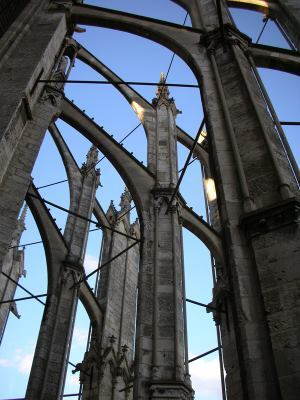
\includegraphics[width=0.8\textwidth]{img/tie-rods-cathedral.jpeg}
                \caption{Steel tie-rods connect the buttresses of the Cathedral of Saint Peter of Beauvais in France. Credit to: \textit{P. Dillmann}.}
            \end{figure}

        \end{column}

    \end{columns}

\end{frame}


\section{Problem statement}

\begin{frame}{Disturbances effect of environmental condition on SHM}

    In case of axial-load beams (tie-rods), studies has highlighted that \textbf{temperature variations can cause greater changes to structural vibration than the presence of damage itself}.

    The transverse vibration in a tensioned beam is described by the following equation\footnotemark[1]:
    \begin{equation}
        w(\xi, t) = \left[ A \sin(\gamma_1 \xi) + B \cos(\gamma_1 \xi) + C \sin(\gamma_2 \xi) + D \cos(\gamma_2 \xi)\right] E \cos(\omega t + \phi)
    \end{equation}

    Where:
    \begin{equation}
        \gamma_1 = \sqrt{\frac{N - \sqrt{N^2 + 4EJ \rho A \omega^2}}{2EJ}} \qquad \gamma_2 = \sqrt{\frac{N + \sqrt{N^2 + 4EJ \rho A \omega^2}}{2EJ}}
    \end{equation}

    Notice that $N = N(Temperature) = N_0 + k (T - T_0)$, with $k \approx -60 \frac{N}{^\circ C}$.

    \footnotetext[1]{A full derivation of the equation can be found in the appendix.}

\end{frame}



\begin{frame}{Formal definition of the problem}

    Both \textcolor[HTML]{FF0000}{Temperature} and \textcolor[HTML]{00B300}{Damage} can affect the eigenfrequency and the mode shape of a structure.

    \begin{figure}
        \centering
        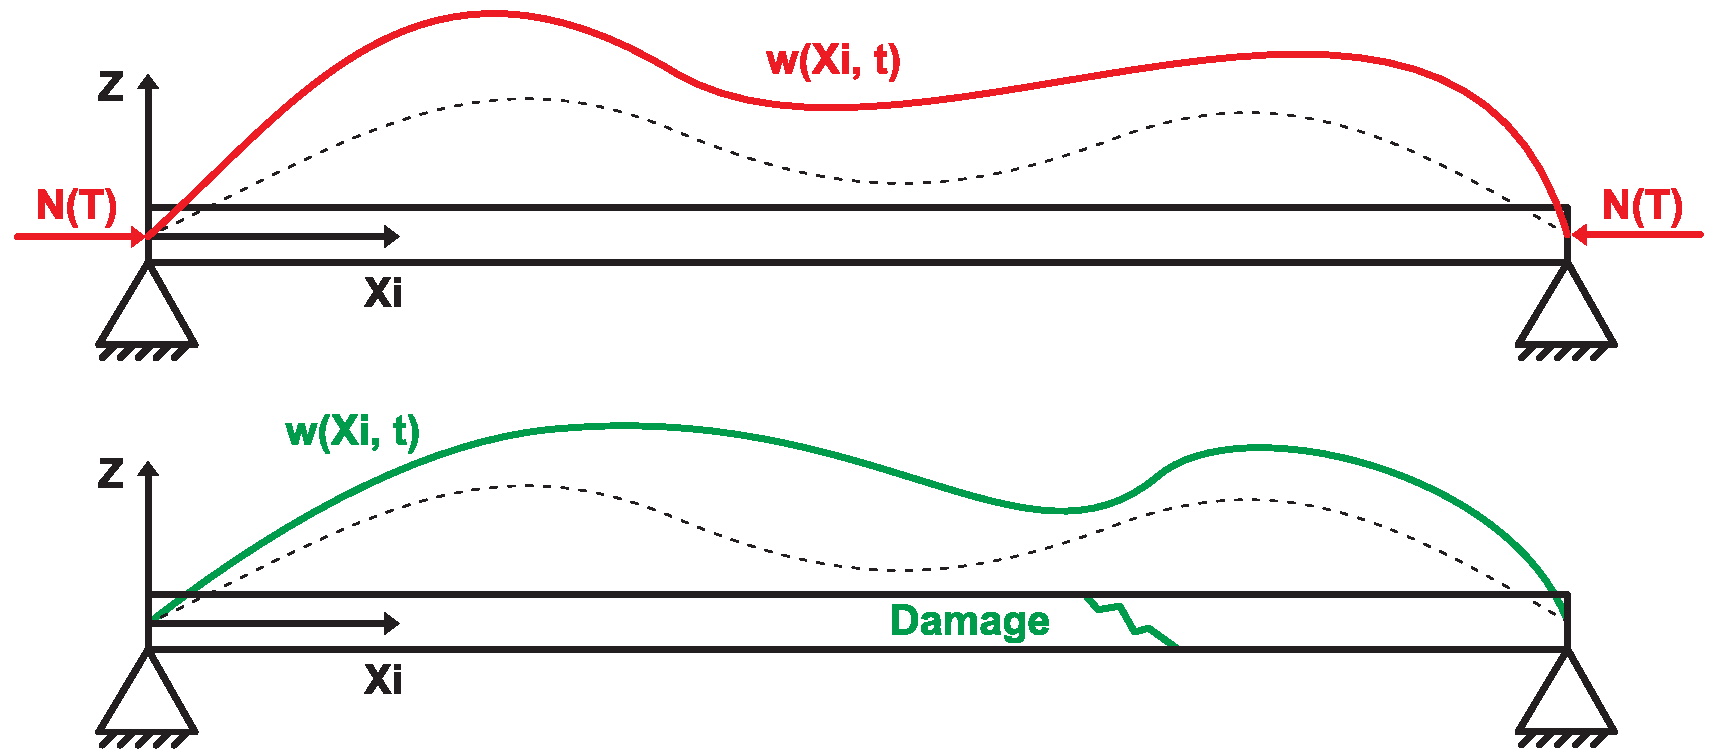
\includegraphics[width=0.8\textwidth]{img/OCAD/tie-rods.pdf}
    \end{figure}

    After a proper OMA\footnotemark[1] analysis, \textbf{how to isolate the effect of environmental condition on the eigenfrequency from the effect of damage?}

    \footnotetext[1]{OMA: Operational Modal Analysis}

\end{frame}
\section{Proposed solutions}

\begin{frame}{Multivariate outlier detection}

    Two \textbf{methods} are presented, both \textbf{based on the concept of multivariate outlier detection in the frequency domain}:

    \begin{itemize}
        \item Mahalanobis Squared Distance (MSD)
        \item Principal Component Analysis (PCA)
    \end{itemize}

\end{frame}



\subsection{Mahalanobis Squared Distance (MSD)}

\begin{frame}{Mahalanobis Squared Distance (MSD) approach}

    The Mahalanobis Squared Distance (MSD) is a measure of the distance between a point and a distribution.


    \begin{columns}[c, onlytextwidth]

        \begin{column}{0.5\textwidth}

            It's defined as:
            \begin{equation}
                D_{MSD}^2 = (\mathbf{x} - \mathbf{\mu})^T \mathbf{\Sigma}^{-1} (\mathbf{x} - \mathbf{\mu})
            \end{equation}

            Where:
            \begin{itemize}
                \item $\mathbf{x}_{(m \times 1)}$ is the vector of the observations
                \item $\mathbf{\mu}_{(m \times 1)}$ is the mean of the observations
                \item $\mathbf{\Sigma}_{(m \times m)}$ is the covariance matrix of the observations
            \end{itemize}

        \end{column}

        \hfill

        \begin{column}{0.45\textwidth}

            \begin{figure}[H]
                \centering
                % https://it.mathworks.com/help/stats/mahal.html
                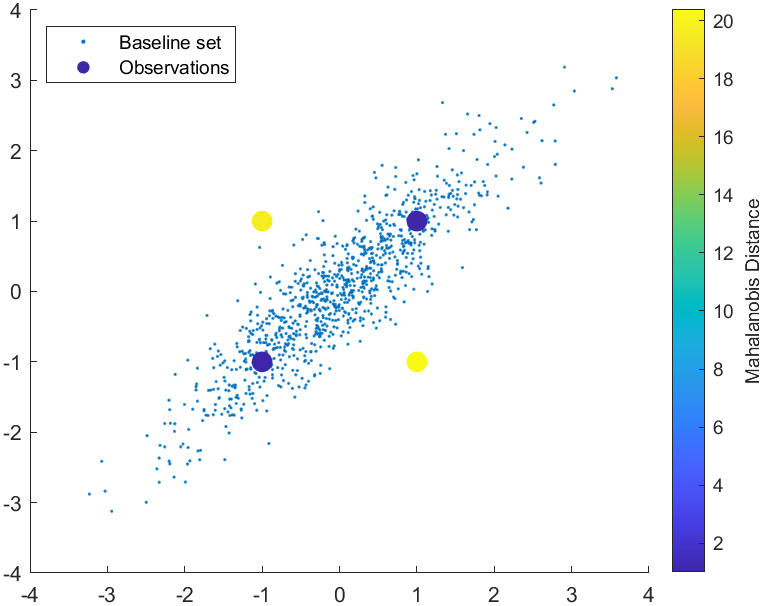
\includegraphics[width=\textwidth]{img/Mahalanobis-cloud-plot.png}
                \caption{Application example of the MSD index. \textcolor[HTML]{F5EC22}{Outliers} are clearly visible. Credit to: \textit{MathWorks}.}
            \end{figure}

        \end{column}

    \end{columns}

    \vspace{9pt}

    The MSD is used to detect outliers in the data, by computing the distance between observations and the distribution of the data.

\end{frame}



\begin{frame}{Issues of the MSD approach related to SHM}

    The MSD approach is \textbf{based on the assumption that the baseline data contains all the possible variations due to environmental effects} (e.g. temperature, vibrations noise, etc.).

    \vspace{9pt}

    To be effective then, the baseline data should be collected in a wide range of environmental conditions in order to capture all the possible variations, \textbf{which imply a long and expensive data collection campaign} that is not always feasible.

\end{frame}



\subsection{Principal Components Analysis (PCA)}

\begin{frame}{Principal Components Analysis (PCA) approach}

    The Principal Components Analysis (PCA) is a statistical method used to project the data onto a new set of coordinate, where the new axes are the principal components of the data. It can also be used to reduce the dimensionality of the problem.

    % https://builtin.com/data-science/step-step-explanation-principal-component-analysis
    \begin{figure}[H]
        \centering
        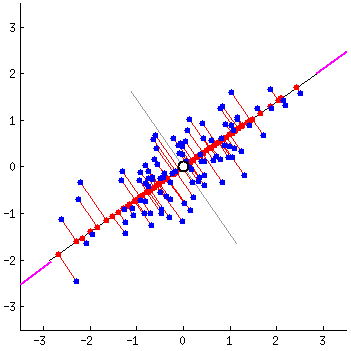
\includegraphics[width=0.3\textwidth]{img/principal-components-01.png}
        \hfill
        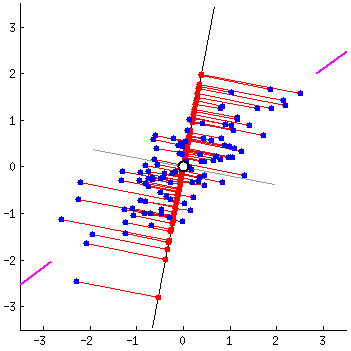
\includegraphics[width=0.3\textwidth]{img/principal-components-02.png}
        \hfill
        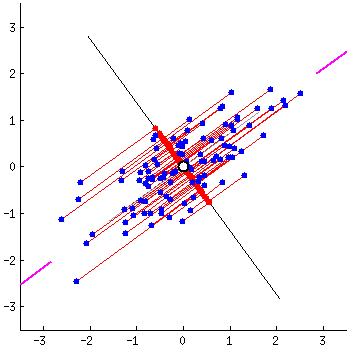
\includegraphics[width=0.3\textwidth]{img/principal-components-03.png}
        \caption{Example of PCA applied to a 2D dataset. PCs are identified as the directions that maximize the variance of the projected cloud of data. With refer to the figures, $1^{st}$ and $3^{rd}$ represent two different PCs configurations, while the $2^{nd}$ mimics the rotational transformation of the data. Credit to: \textit{Z. Jaadi}.}
    \end{figure}

    In a broad sense, the result of the PCA can be interpreted ad the `eigenvectors' of the cloud of data.

\end{frame}



\begin{frame}{Singular Value Decomposition (SVD) in the PCA approach}

    The Singular Value Decomposition (SVD) is a mathematical technique used to compute the rotational transformation needed to project the data onto the principal components.

    By definition, SVD of a matrix $\mathbf{A}_{(n \times m)}$ is defined as:

    \begin{equation}
        \mathbf{A} = \mathbf{U} \mathbf{\Sigma} \mathbf{V}^T
    \end{equation}

    Where:
    \begin{itemize}
        \item $\mathbf{U}_{(n \times n)}$ is the matrix of the left singular vectors of $\mathbf{A}$
        \item $\mathbf{\Sigma}_{(n \times m)}$ is the diagonal matrix of the singular values of $\mathbf{A}$
        \item $\mathbf{V}_{(m \times m)}$ is the matrix of the right singular vectors of $\mathbf{A}$
    \end{itemize}

    \vspace{9pt}

    Finally, the original data can be projected onto the principal components directions by means of the following transformation:
    \begin{equation}
        \mathbf{\hat{A}} = \mathbf{A} \mathbf{V}
    \end{equation}

\end{frame}



\begin{frame}{Analysis of signals via PCA}

    The clear decreasing trend of the deterministic amount, suggests that only the first(s) principal component(s) are affected by environmental conditions.
    By removing them, \textbf{we can analyze the remaining components that are likely to be strictly related to the damage itself}.

    \begin{figure}
        \centering
        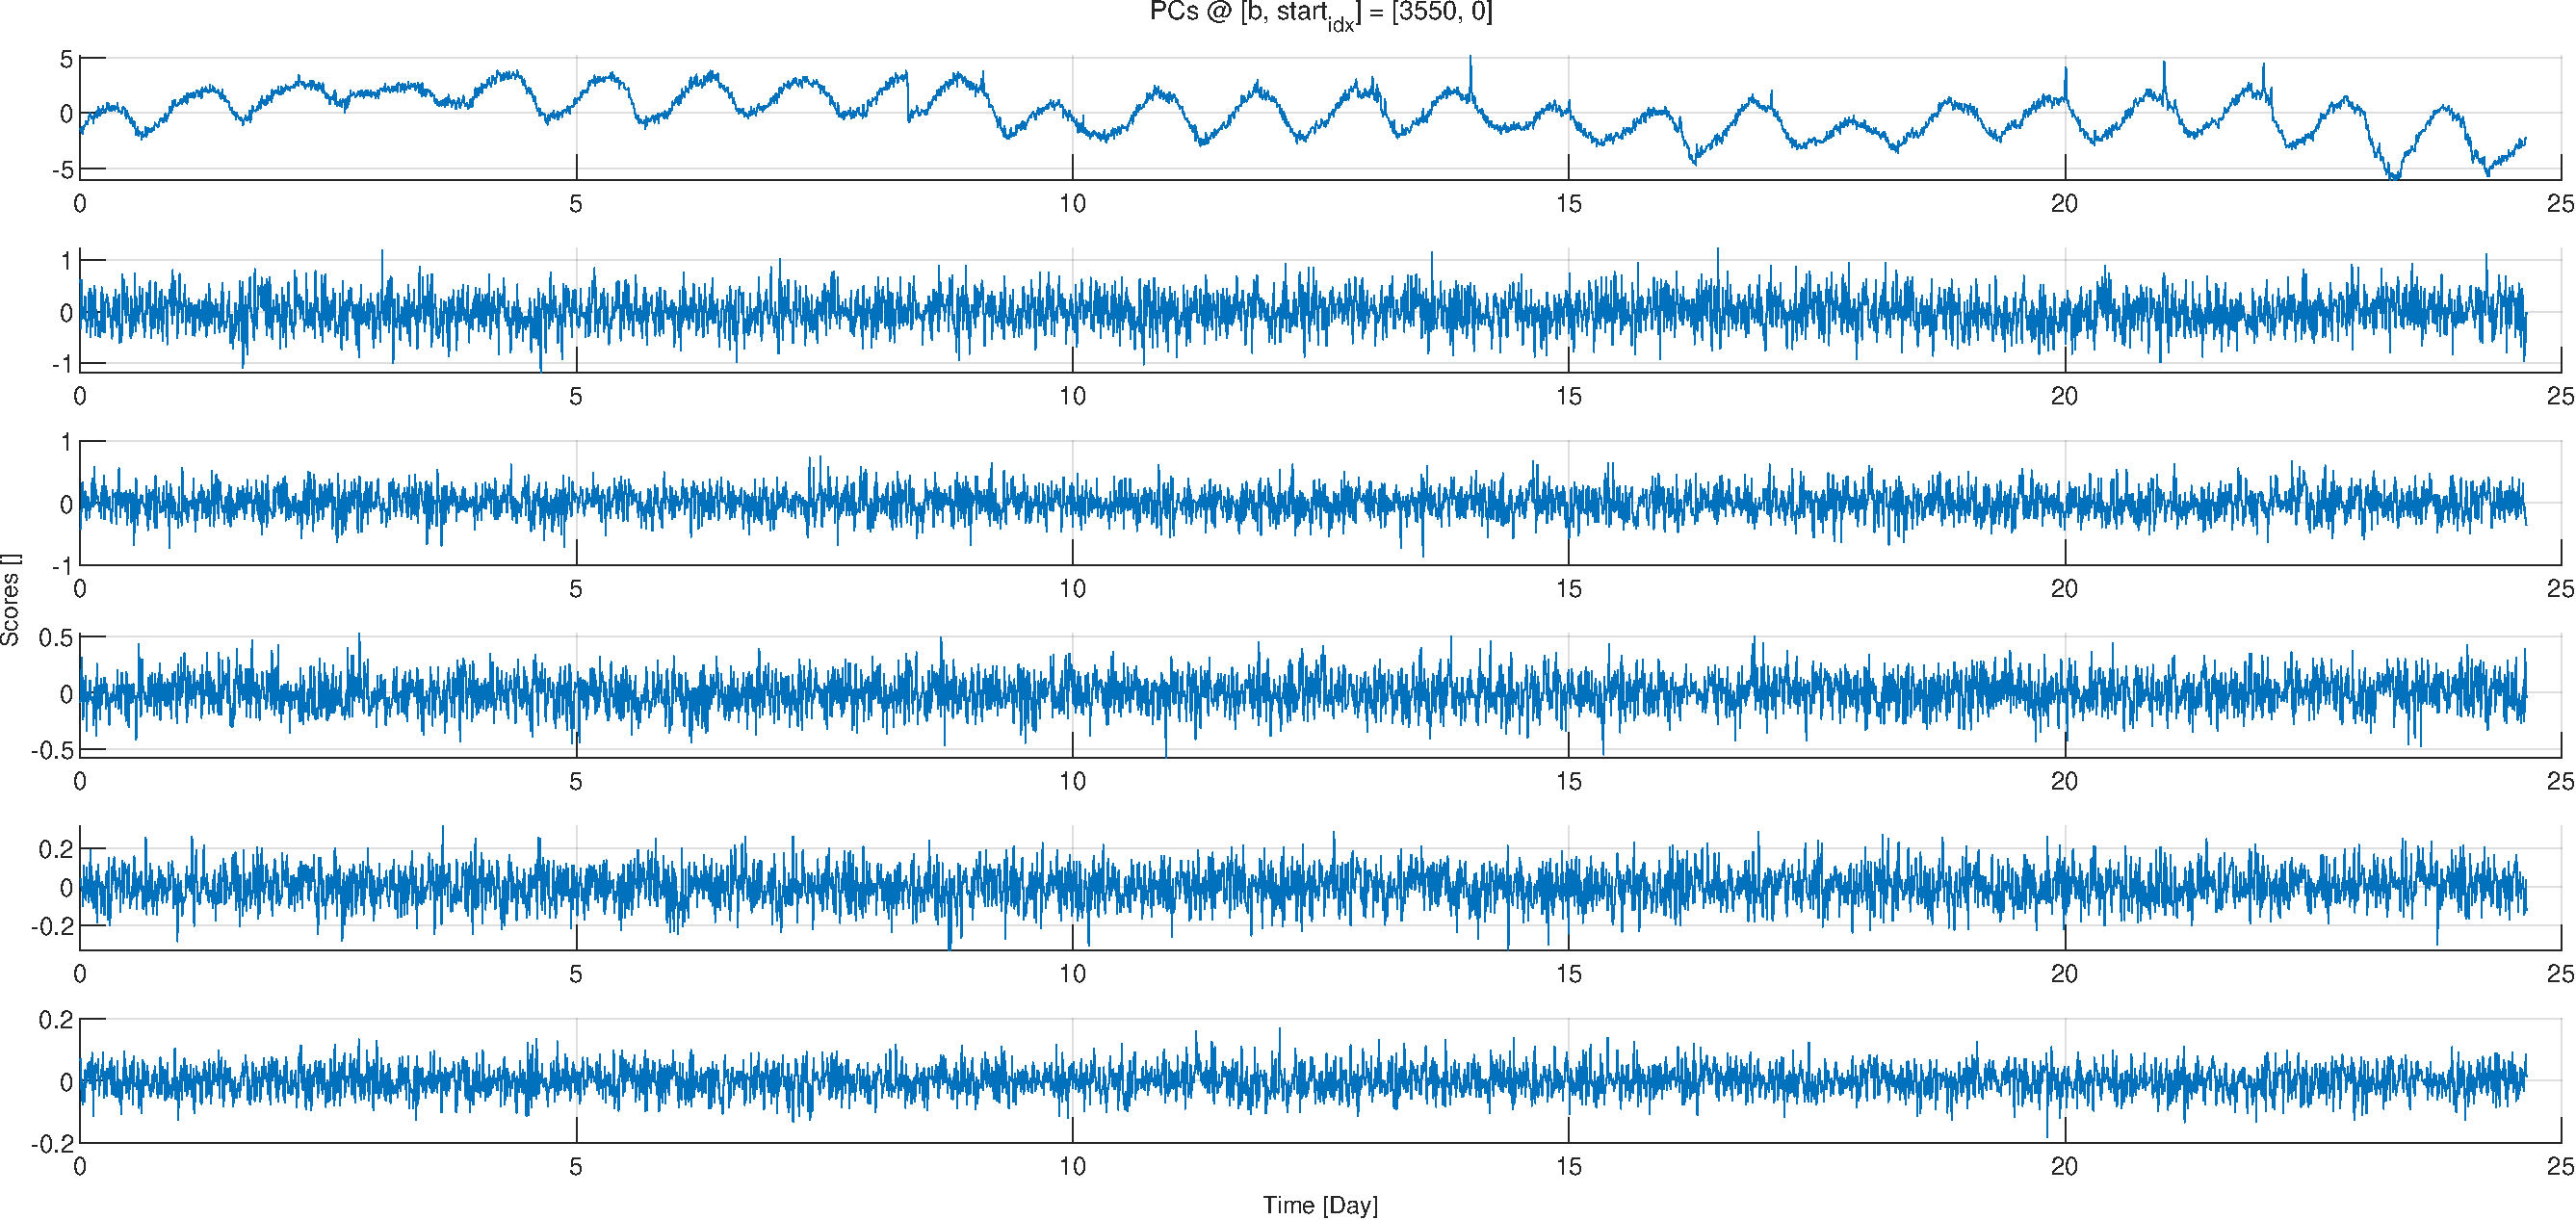
\includegraphics[width=0.9\textwidth]{img/MATLAB/PCs_01.pdf}
        \caption{Scores of the eigenfrequencies of the structure projected onto the principal components. Here, $b = 20\% \times data_{length} = 3550$.}
    \end{figure}

\end{frame}
\section{Results}

\begin{frame}{MSD vs. PCA - Baseline set length ($b$)}

    Here we observe the effect of the baseline set length $b$ on the accuracy of the two methods.

    \begin{figure}[H]
        \centering
        \only<1>{
            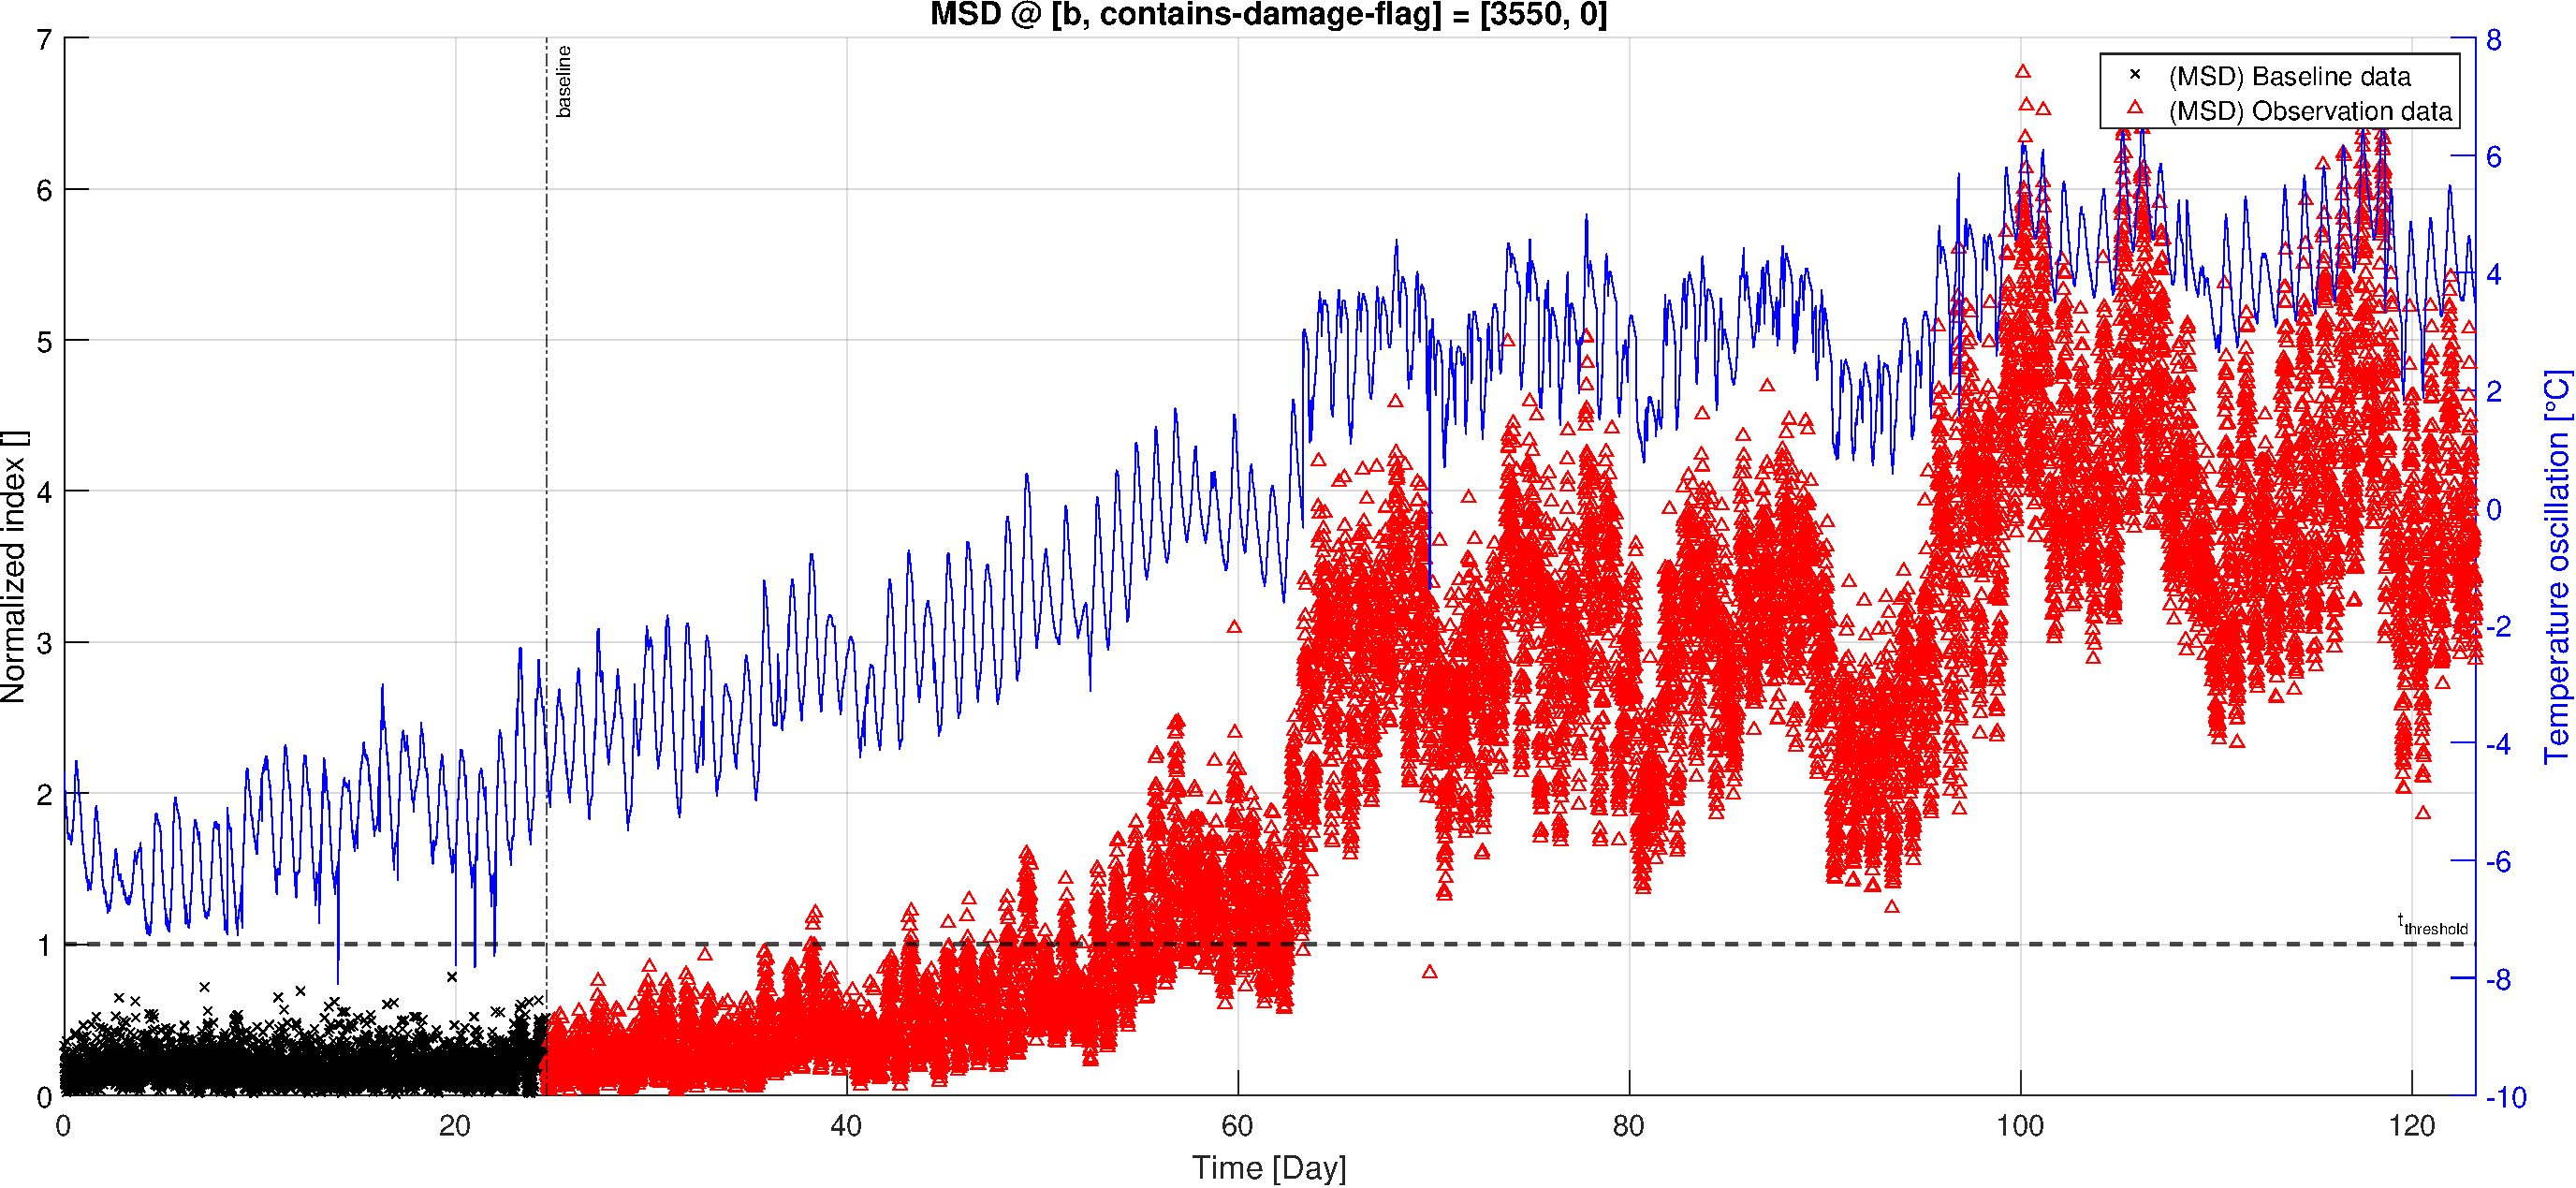
\includegraphics[width=0.9\textwidth]{img/Baseline/MSD_Baseline_3550.pdf}
            \caption{MSD method considering $b = 3550$}
        }
        \only<2>{
            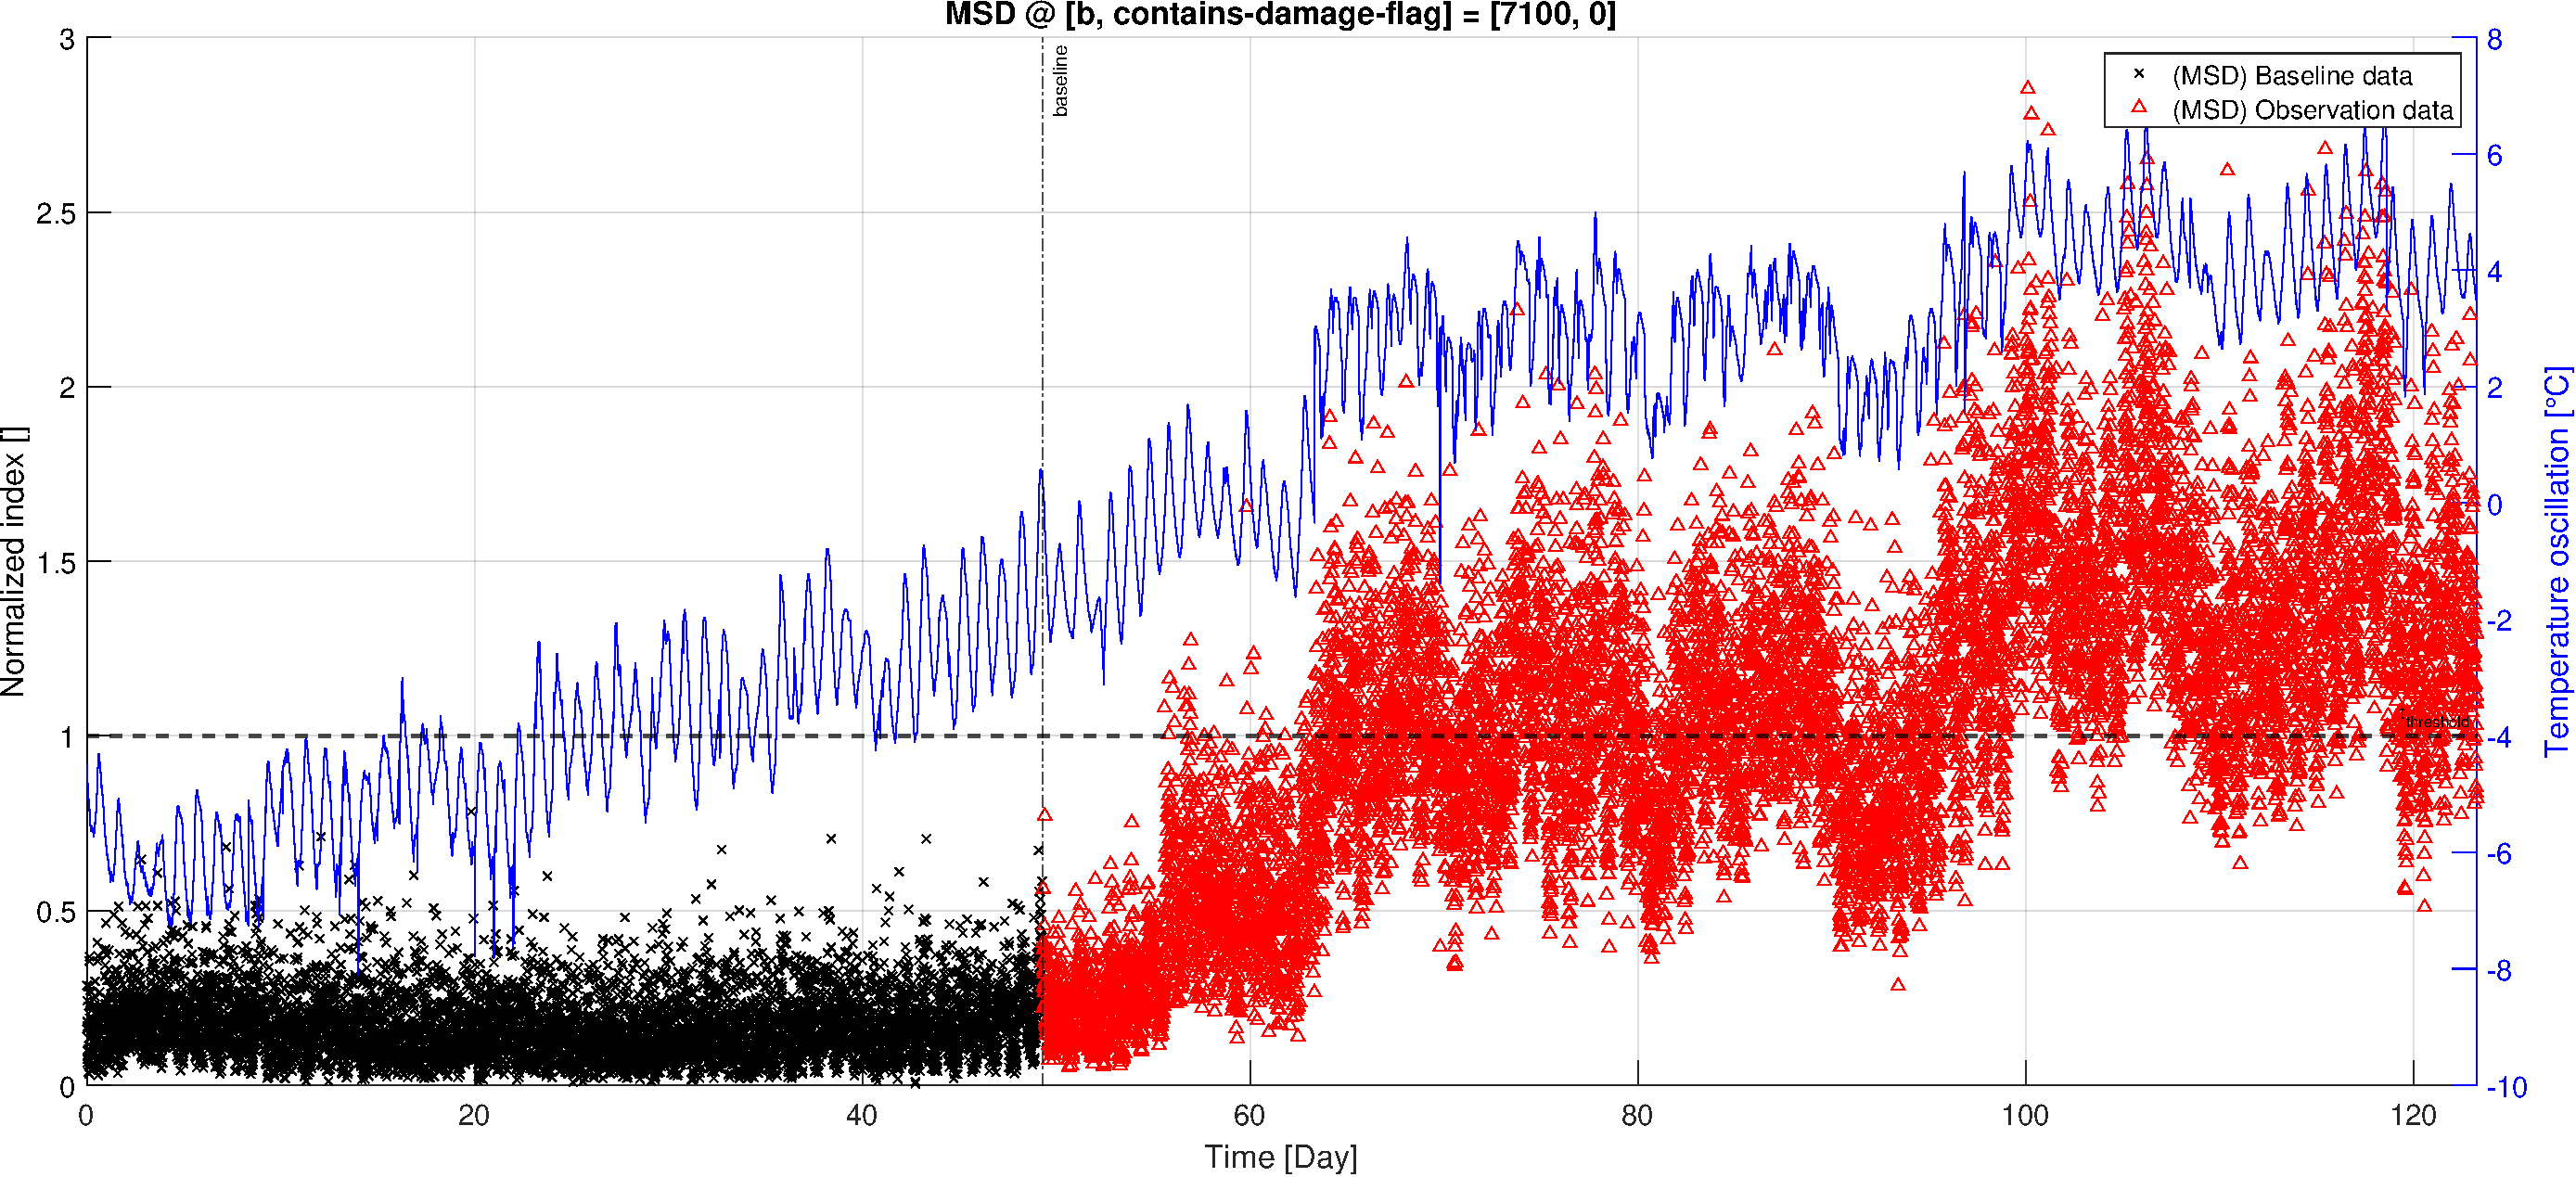
\includegraphics[width=0.9\textwidth]{img/Baseline/MSD_Baseline_7100.pdf}
            \caption{MSD method considering $b = 7100$}
        }
        \only<3>{
            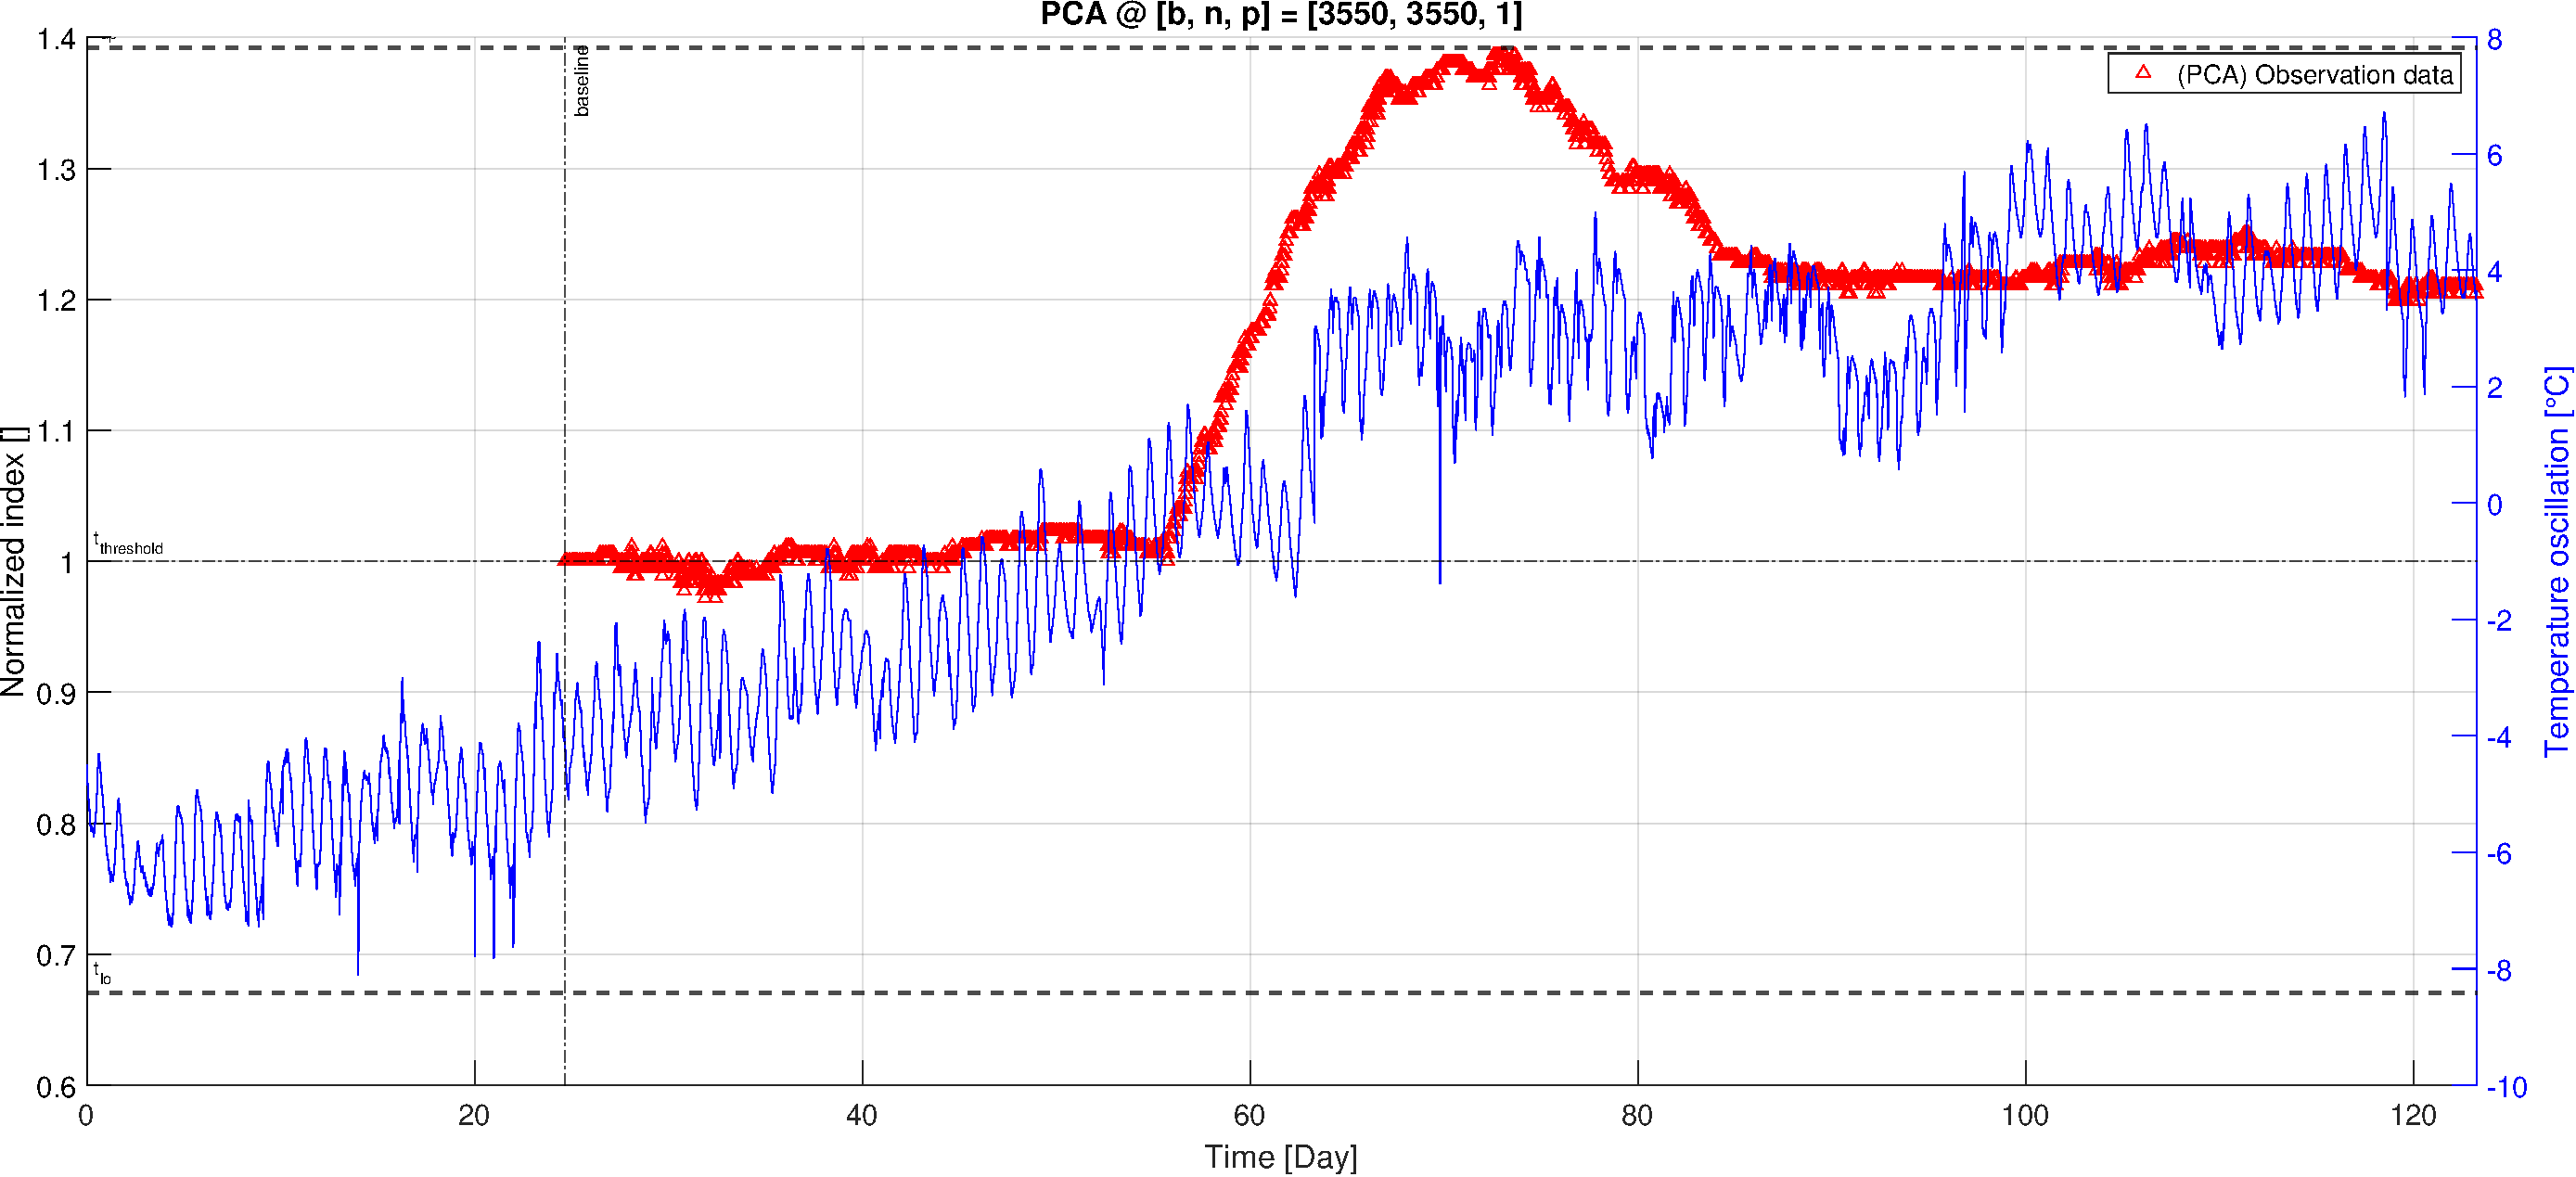
\includegraphics[width=0.9\textwidth]{img/Baseline/PCA_Baseline_3550.pdf}
            \caption{PCA method considering $b = n = 3550$}
        }
        \only<4>{
            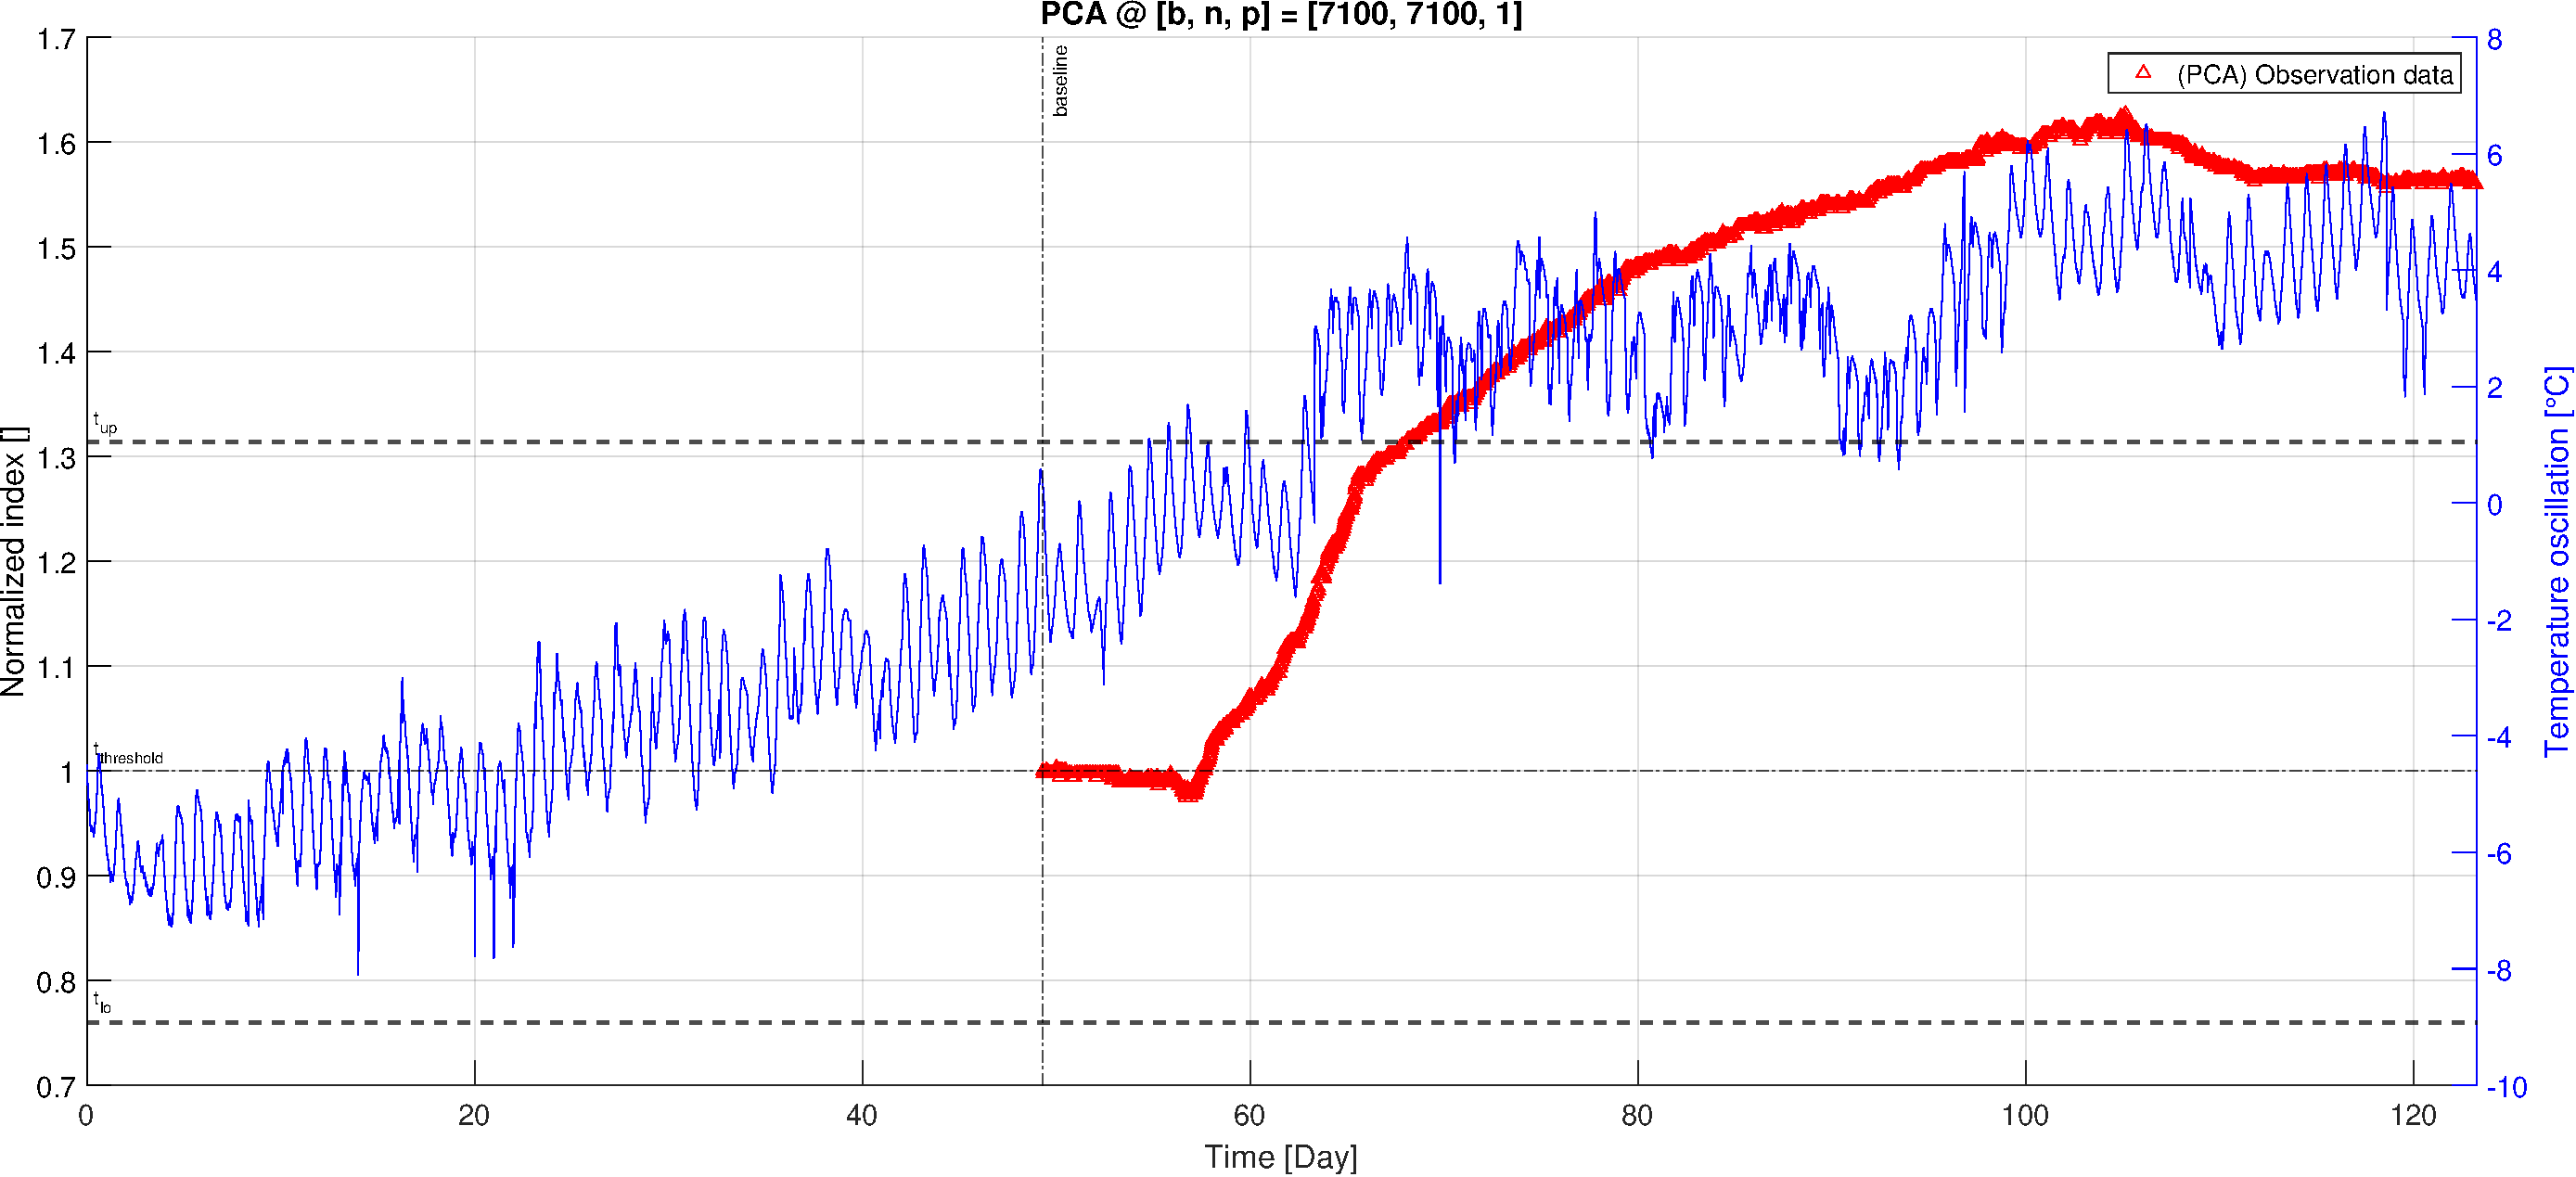
\includegraphics[width=0.9\textwidth]{img/Baseline/PCA_Baseline_7100.pdf}
            \caption{PCA method considering $b = n = 7100$}
        }
    \end{figure}

    \vspace{-9pt}

    \only<1,2>{
        The MSD method is highly sensitive to $b$ and if the baseline set doesn't contain a complete set of environmental conditions, it may lead to false positives/negatives.
    }

    \only<3,4>{
        The PCA method, instead, is able to detect outliers (almost) independently of the baseline set length, thus shorter campaigns can be performed without losing accuracy.
    }

\end{frame}



\begin{frame}{PCA - Observation window length ($n$)}

    A key difference between the MSD and PCA methods is that MSD compute the index for each observation record, while PCA computes the index for a set of records with length $n$.

    \begin{figure}[H]
        \centering
        \only<1>{
            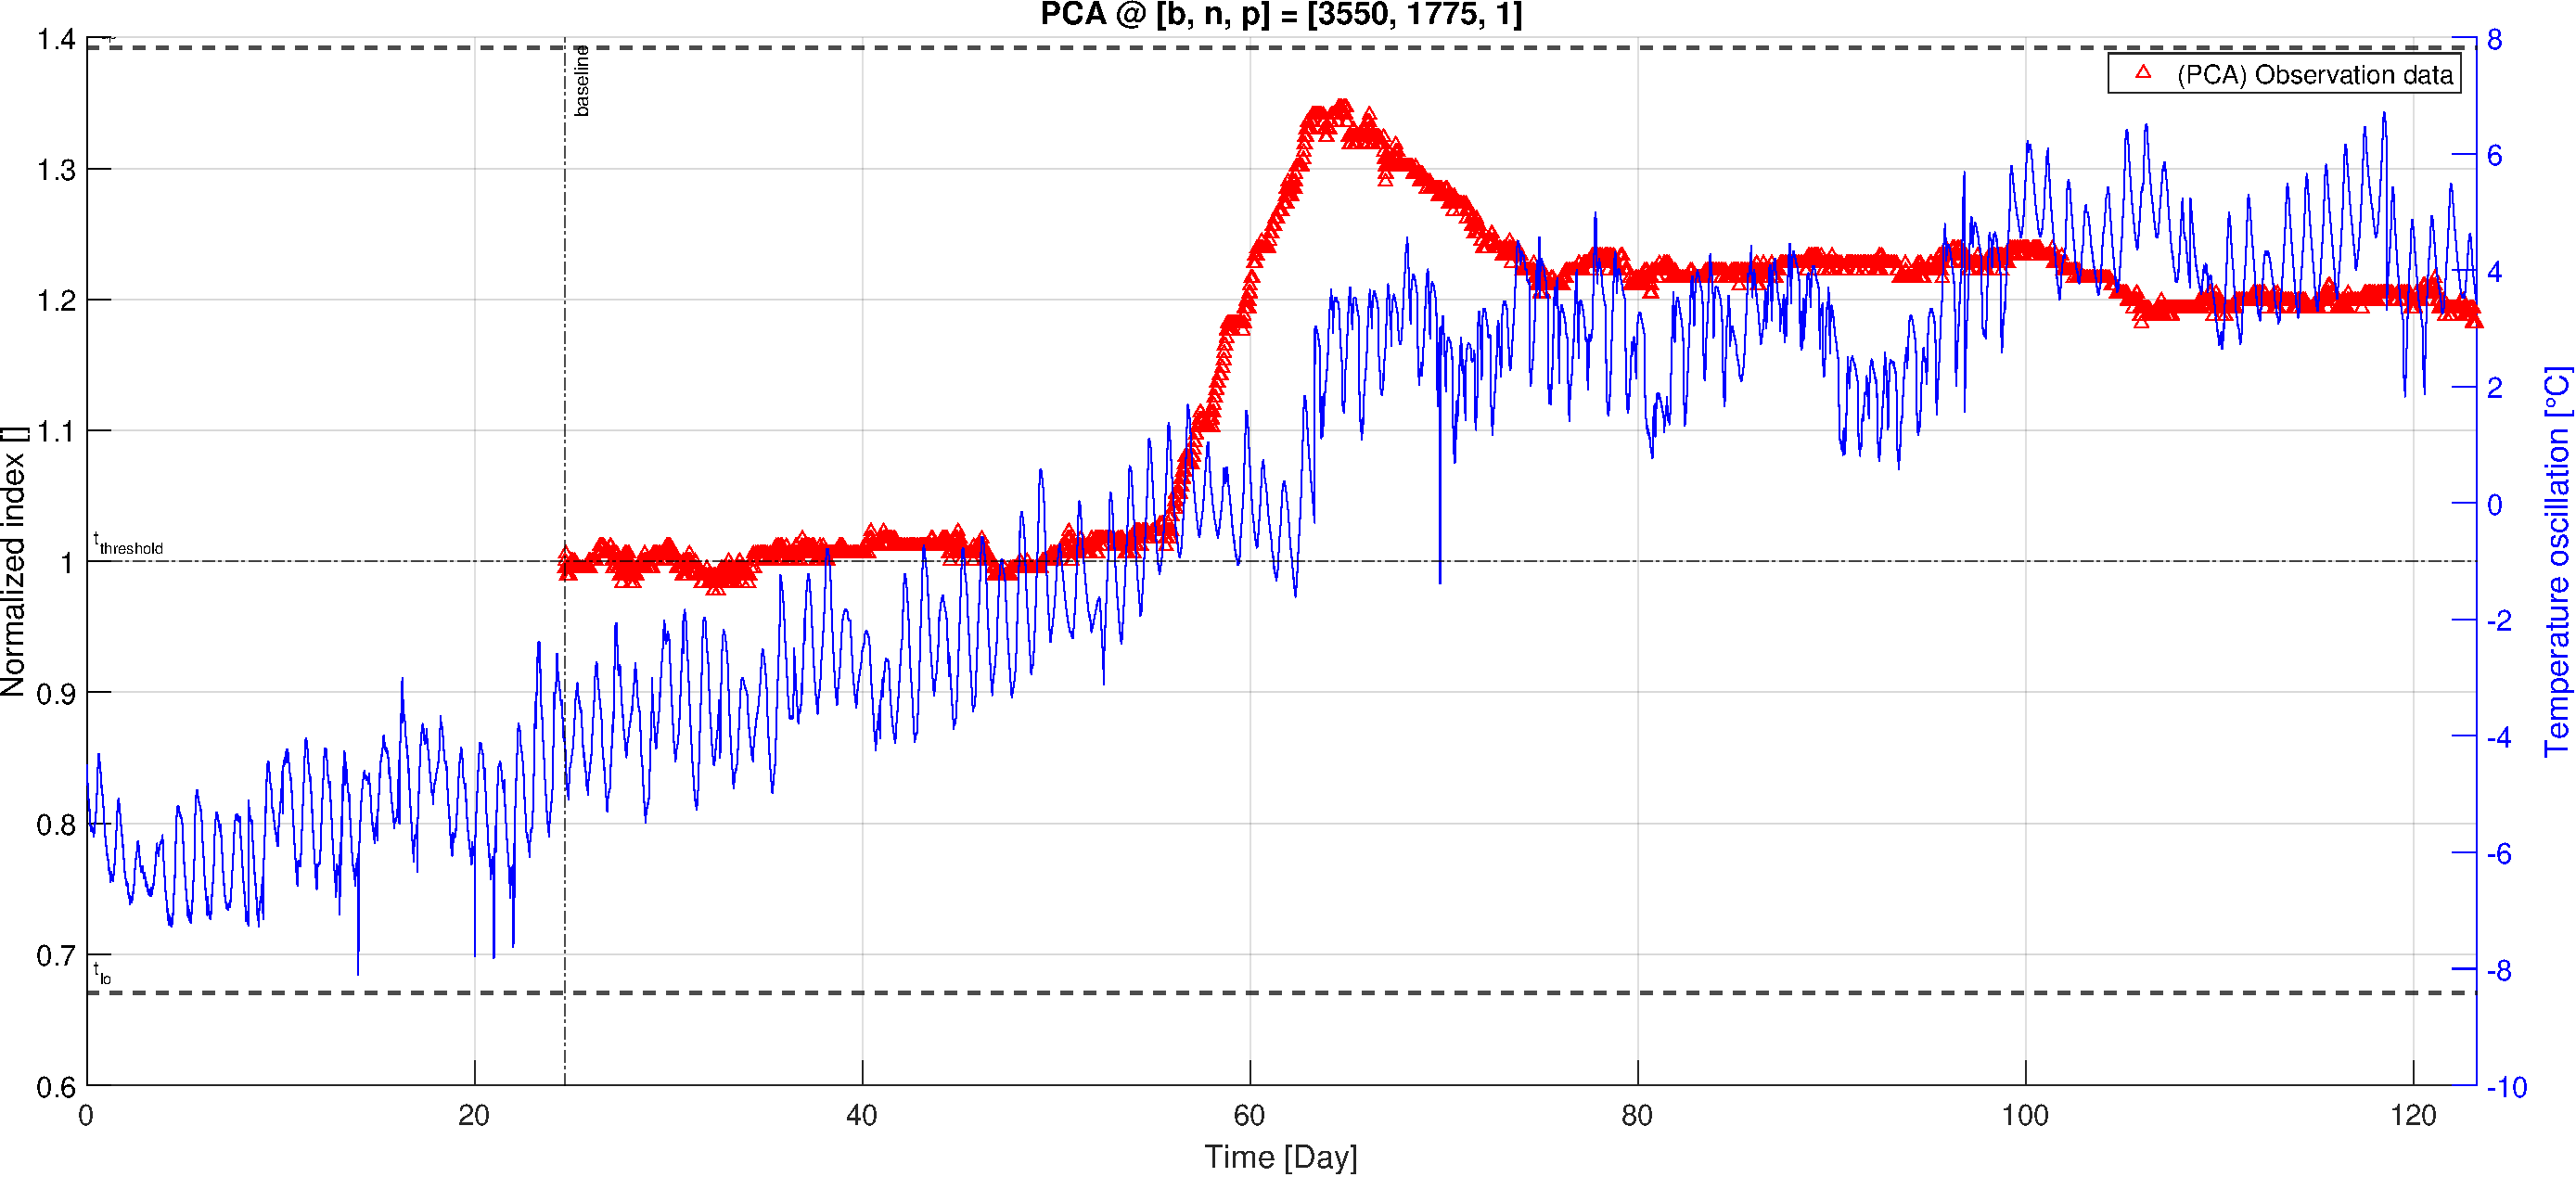
\includegraphics[width=0.9\textwidth]{img/Window/PCA_Window_1775.pdf}
            \caption{PCA method considering $b = 3550$ \& $n = 1775$}
        }
        \only<2>{
            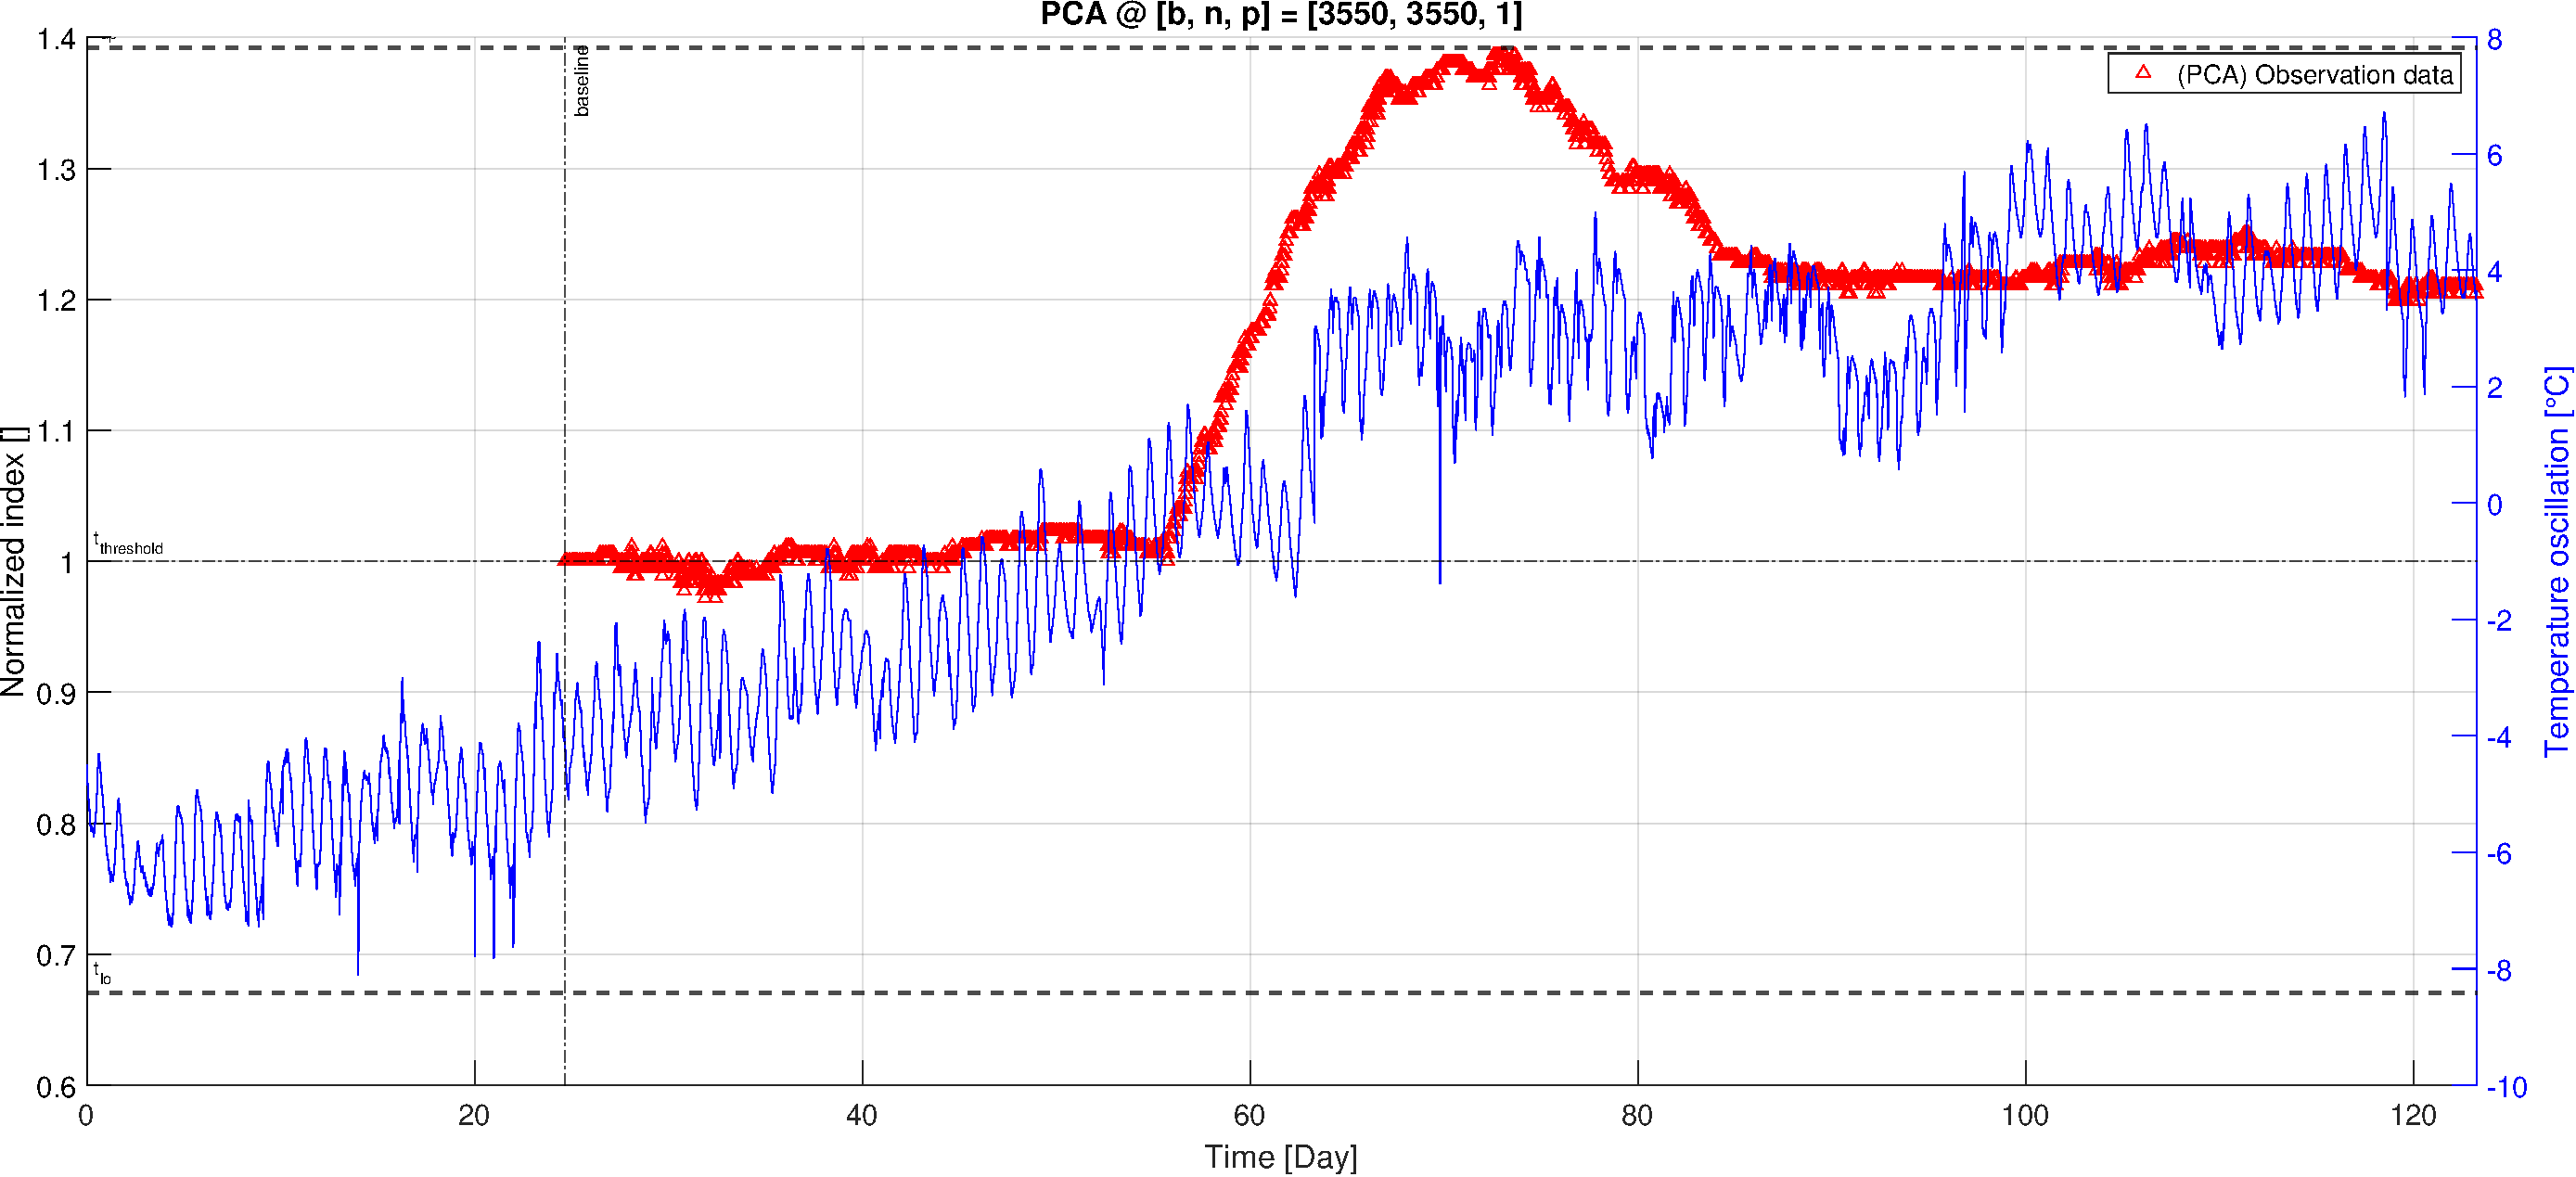
\includegraphics[width=0.9\textwidth]{img/Window/PCA_Window_3550.pdf}
            \caption{PCA method considering $b = 3550$ \& $n = 3550$}
        }
        \only<3>{
            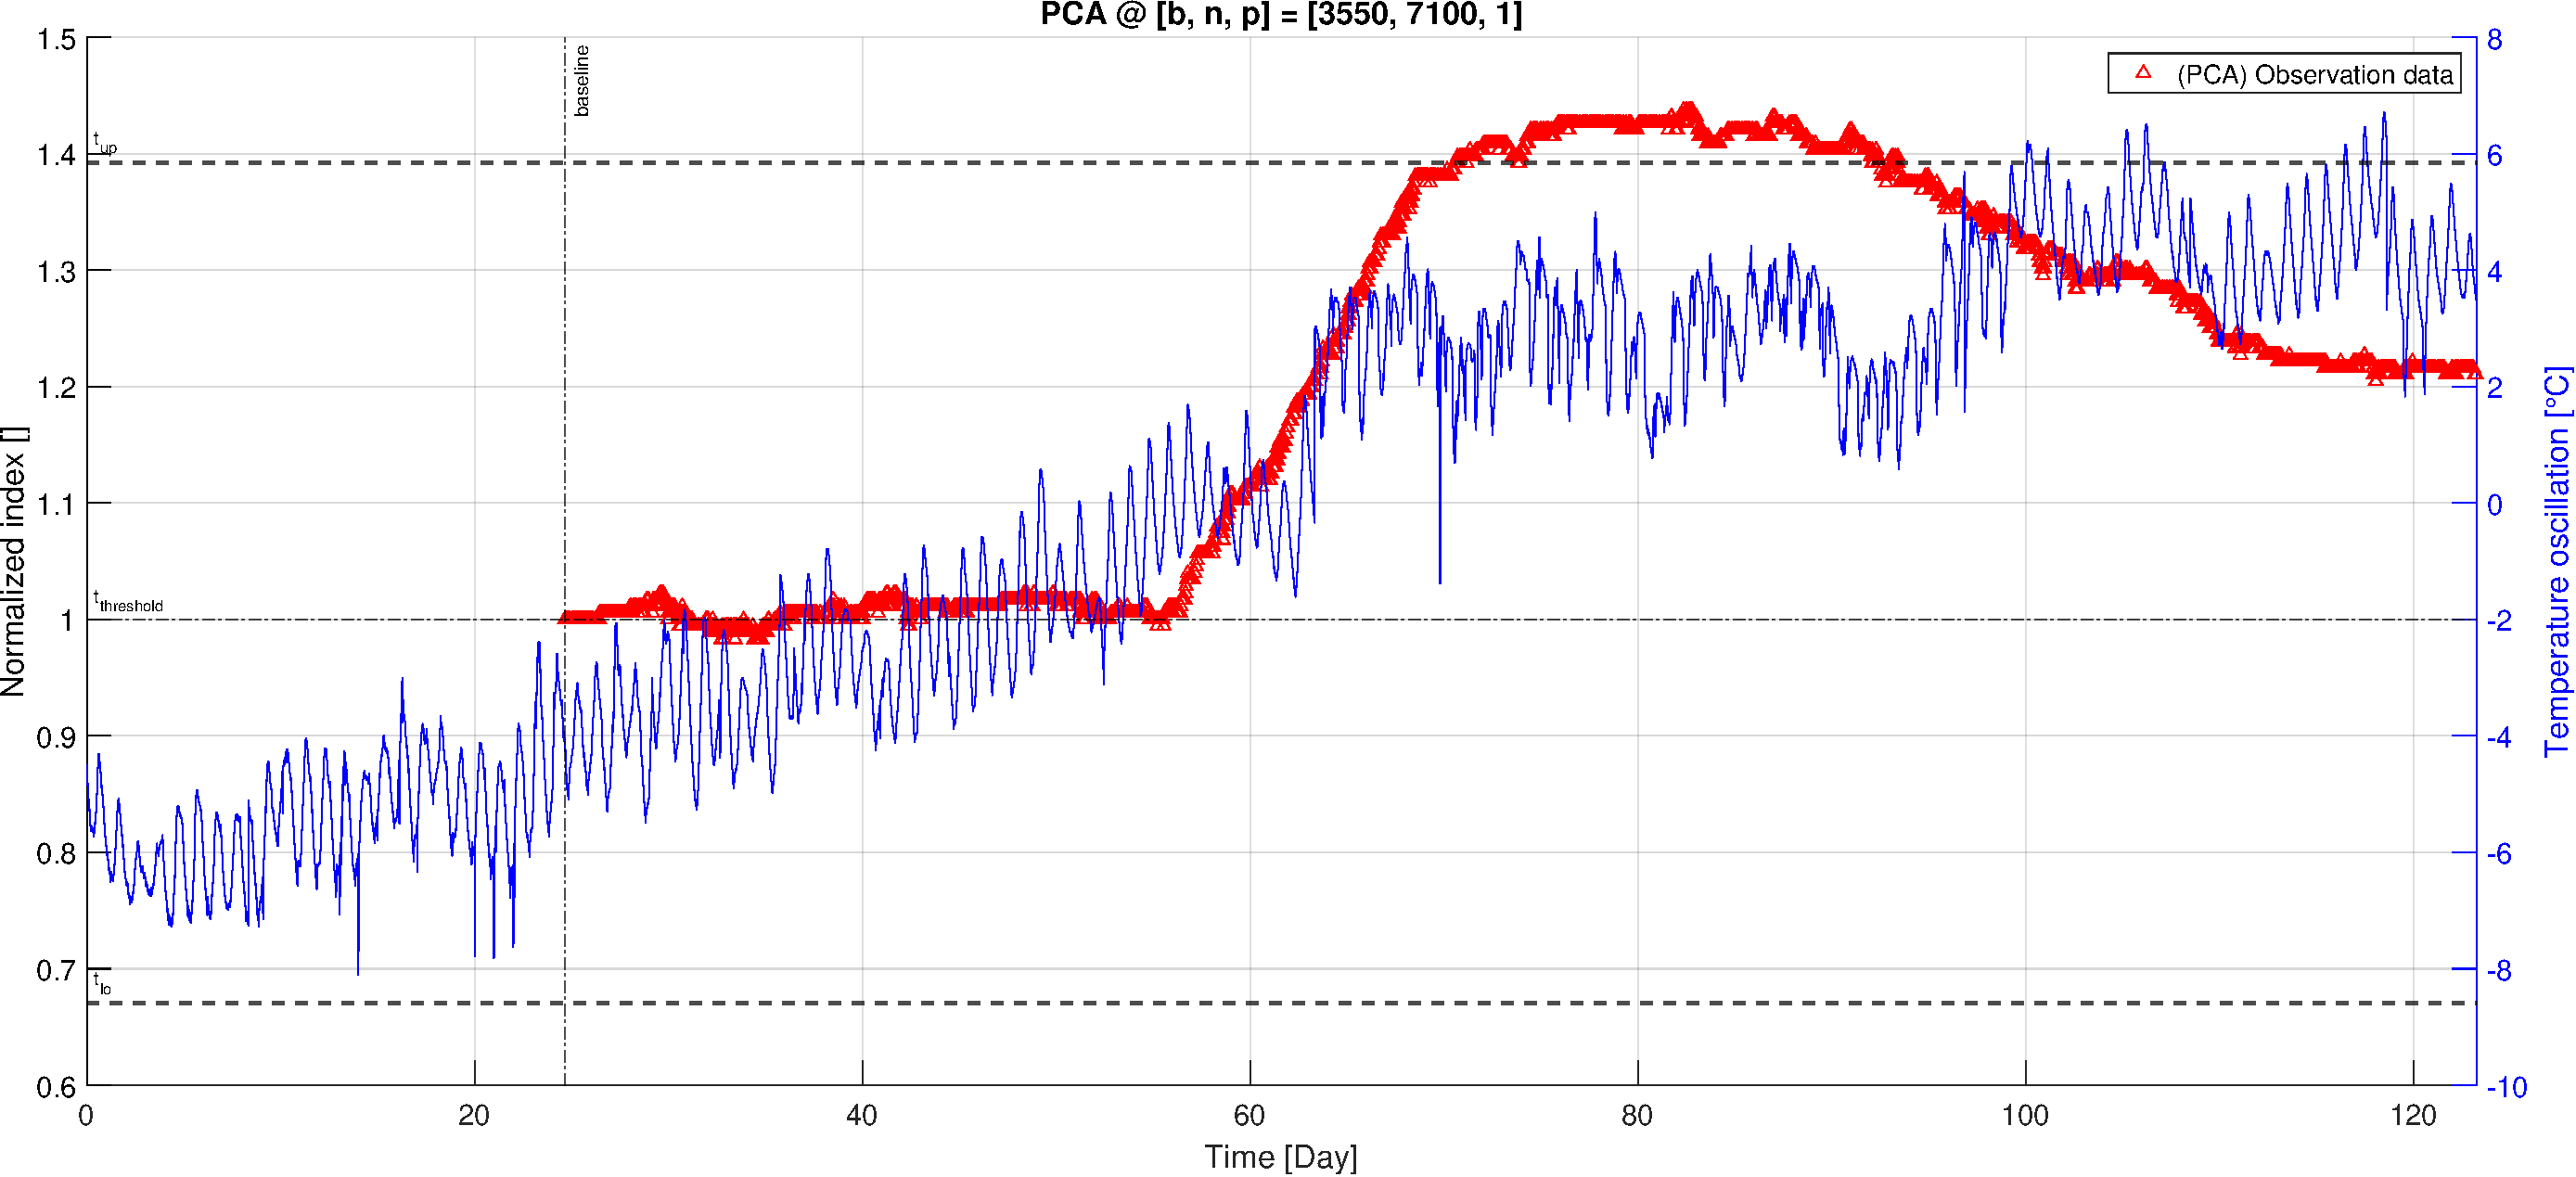
\includegraphics[width=0.9\textwidth]{img/Window/PCA_Window_7100.pdf}
            \caption{PCA method considering $b = 3550$ \& $n = 7100$}
        }
        \only<4>{
            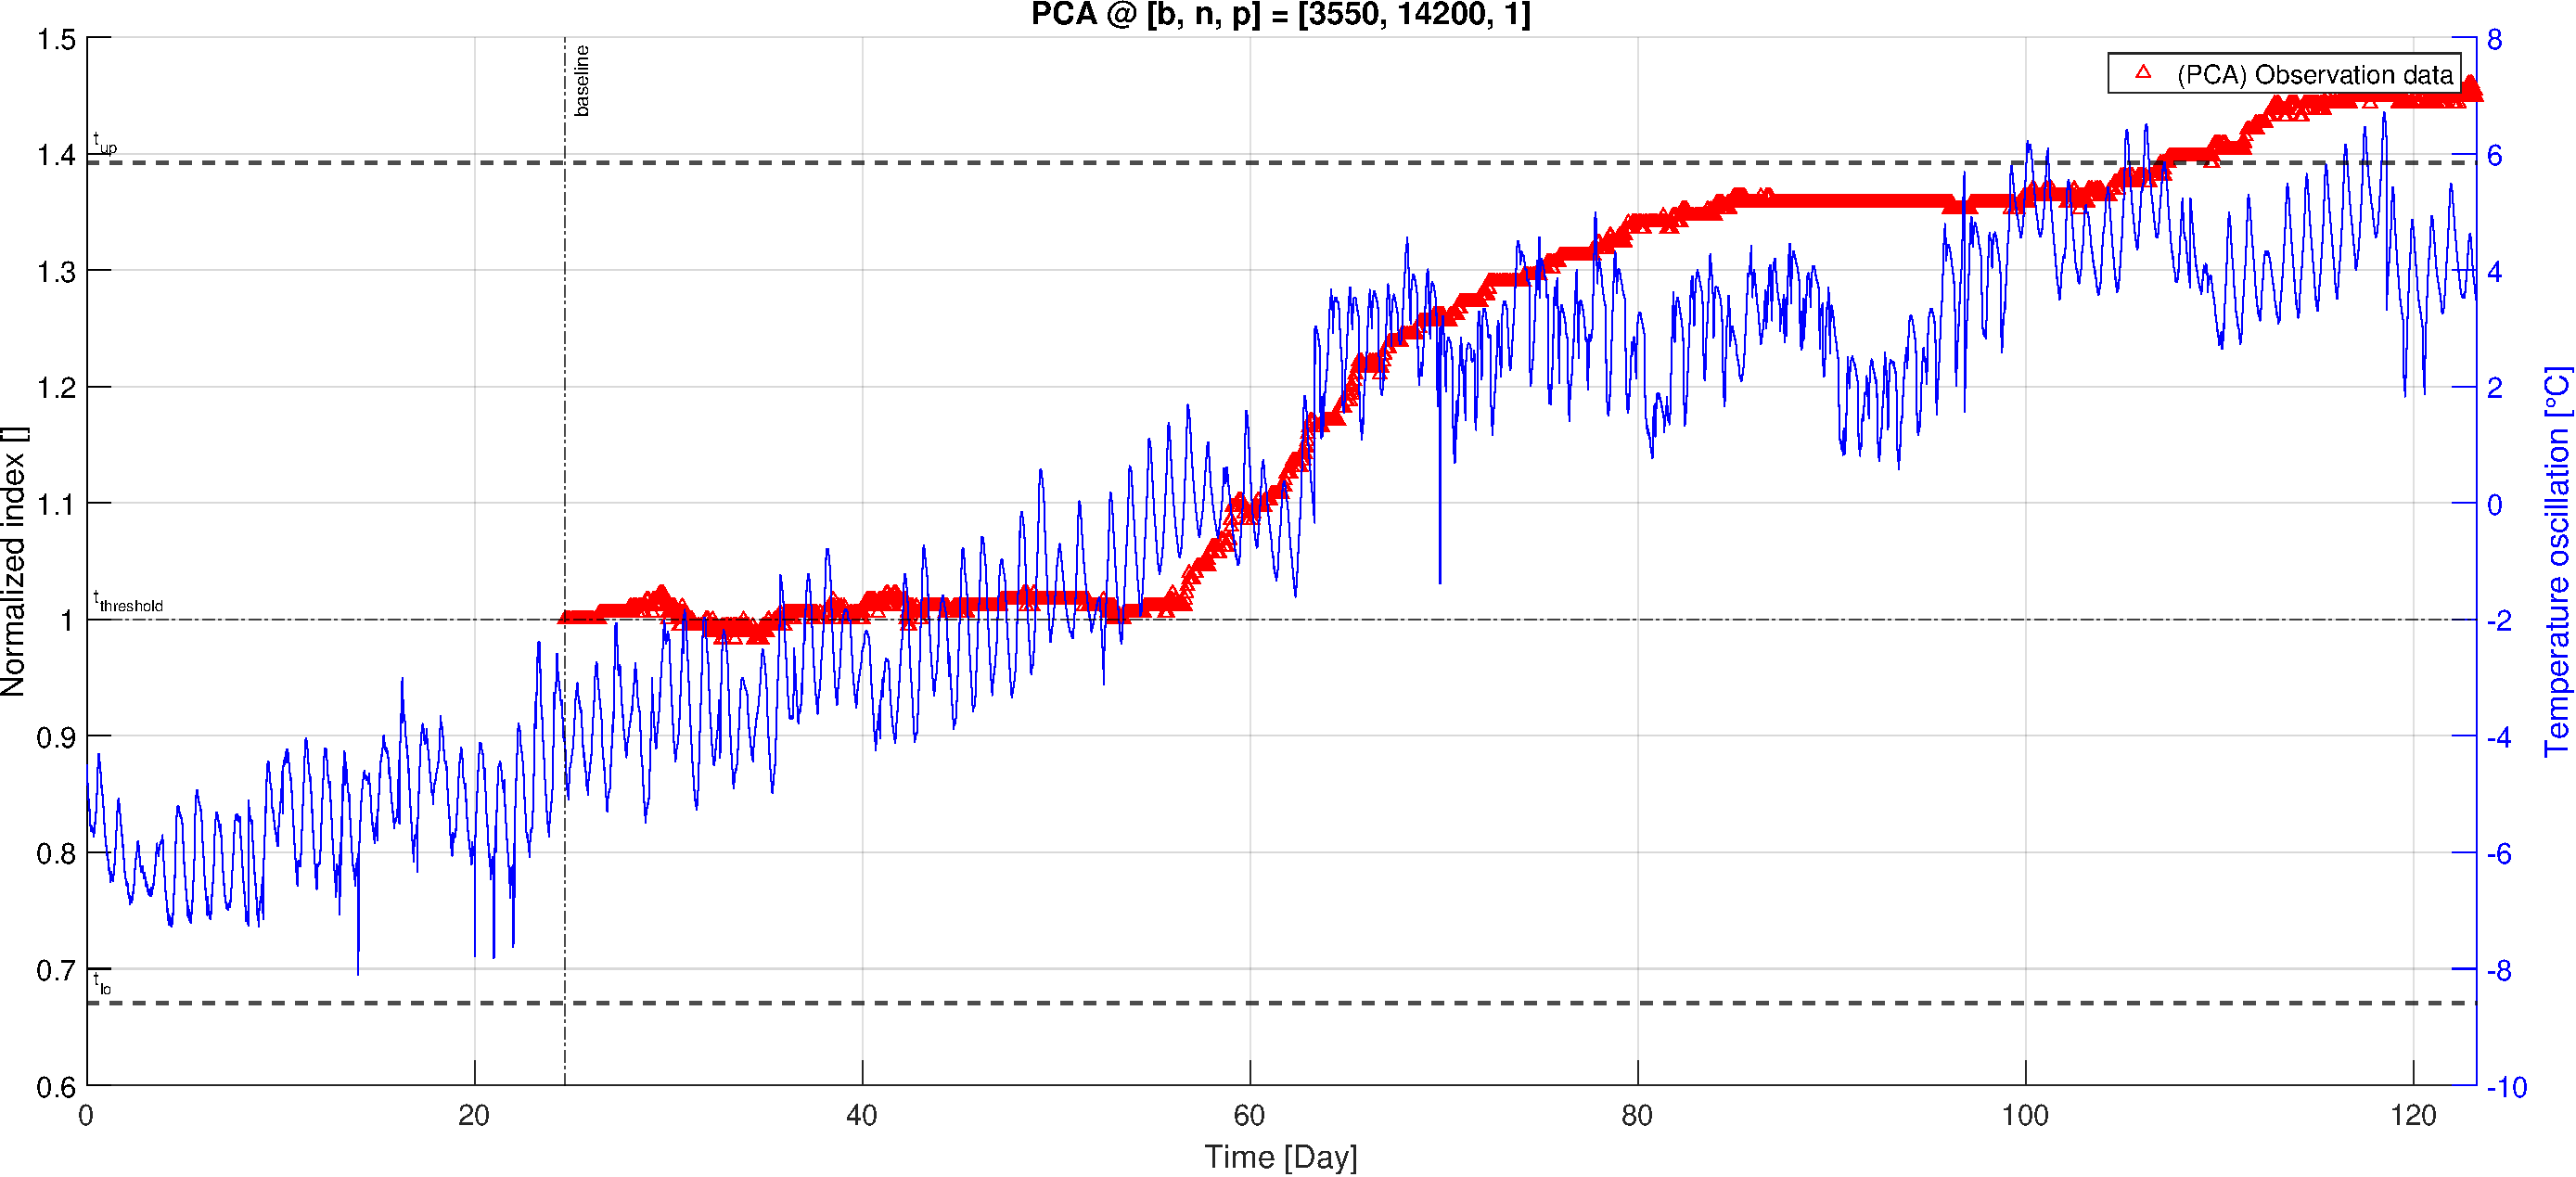
\includegraphics[width=0.9\textwidth]{img/Window/PCA_Window_14200.pdf}
            \caption{PCA method considering $b = 3550$ \& $n = 14200$}
        }
    \end{figure}

    \vspace{-9pt}

    It's clear how $n$ affect the reactivity of the PCA method to detect outliers.
    In particular, the higher $n$, the slower the transient response of the index.

\end{frame}
\section{Conclusions}

\begin{frame}{Method comparison}

    Overall, both the proposed approaches has shown to be effective in detecting damage in the tie-rods.

    However, the use of the PCA methods offers some non-negligible advantages:

    \begin{itemize}
        \item It's more robust in isolate the damage features from other sources of variability.
        \item It doesn't require a training set that includes all the possible environmental conditions, thus eliminating the need for a long data sampling campaign.
    \end{itemize}

\end{frame}



\begin{frame}{Future work and preliminary solutions}

    Regarding the PCA method, some possible future developments and solutions spotted during the research are:

    \begin{table}
        \centering
        \begin{tabular}{l|l}
            \textbf{Future work}  & \textbf{Preliminary solution}                                                        \\
            \hline
            Automatic PCs removal & Set a threshold based on an RMS of each PCs and remove the PC that exceed this limit \\
            \hline
        \end{tabular}
    \end{table}

\end{frame}
% \begin{frame}[standout]
    Extra slides
\end{frame}



\begin{frame}{Title}

\end{frame}

\appendix

\begin{frame}[allowframebreaks]{References}
    \nocite{*}
    \bibliography{references}
\end{frame}

\begin{frame}[standout]
    Questions?
\end{frame}

\begin{frame}[standout]
    Thank you!
\end{frame}

\end{document}